\section{Introduction}
Artificial intelligence (AI) can analyze large amounts
of data and solve complex problems in various fields.
Most existing state of the art AI techniques rely on
rich and high-quality datasets to train a highly accurate
machine learning model. For example, while training
the SAM model, Alexander et al.~\cite{kirillov2023segment} build the largest
segmented dataset ever, building more than 1 billion
masks on 11 million images. However, in practical reality,
most companies cannot construct such large and highquality datasets as Meta when training their model. To
address this problem, one possible solution is the sharing
of data among multiple organizations or companies to
collaboratively train models.

But collaborative training presents several new challenges while collaborative training has developed rapidly.
The first challenge stems from data privacy. The data held
by organizations may contain sensitive information, such
as medical or financial data of their users. Additionally,
new legal frameworks are increasingly emphasizing the
protection of individual data privacy~\cite{voigt2017eu}. Privacy protection introduces restrictions that prevent privacy data from
leaving its originating organization and being uploaded
to central server. The second challenge is related to the
diverse organizations of data. Data from different organizations provides an increase in available data, driving
advancements in artificial intelligence models. However,
due to the various organizations, storing and processing
data from different organizations, as well as reducing communication costs between these organizations have
become new challenge to overcome.

\begin{figure}[t]
    \centering
  
    \includegraphics[width=1.0\linewidth,height=2.5in]{output/fig1.eps}
     \caption{A schematic of federated learning. Arrow 1 represents the
     central server sending the initialized global model to the client. The
     clients then train locally and submit the local updates to the server
     (arrow 2). The server performs the model aggregation (arrow 3). And
     the server sends the aggregated model to the clients (arrow 4).}
     \label{fig1}
\end{figure}

In response to such challenges, Google [3] develops a
distributed machine learning framework called federated
learning (FL). This framework allows each client to collectively train models without sharing their data. The data
of each client remains private and inaccessible to others
during training process. As shown in Fig.1, in a typical federated learning framework, the server firstly sends a global
model to all selected clients as local models. These clients
then use their local datasets to train the local models and
upload their trained model updates to the central server.
After receiving the updates from all selected clients, the
server updates the global model by averaging the uploaded
updates. And the server sends the updated global model
to the selected clients. After the four steps, one iteration
of federated learning is complete. The entire federated
learning requires multiple iterations to make model achieve
convergence. Throughout the training process, only the
data owners have access to their local data. This approach
ensures the protection of data from unauthorized access
by other clients or the central server, while also reducing
communication costs between the clients and the server
[4]. Due to the clear advantages of FL, FL has been widely
applied to many fields in recent years [5]–[10]. However,
further research has shown that federated learning also
faces numerous security risks [11]–[15], such as backdoor
attacks, adversarial attacks, and Byzantine attacks. The distributed nature of federated learning clients makes it
more challenging to guarantee the trustworthiness of each
client. Consequently, compared to traditional centralized
machine learning, federated learning is more susceptible
to attacks [11]. So there are many researchs on defenses.


\begin{figure}[t]
    \centering
    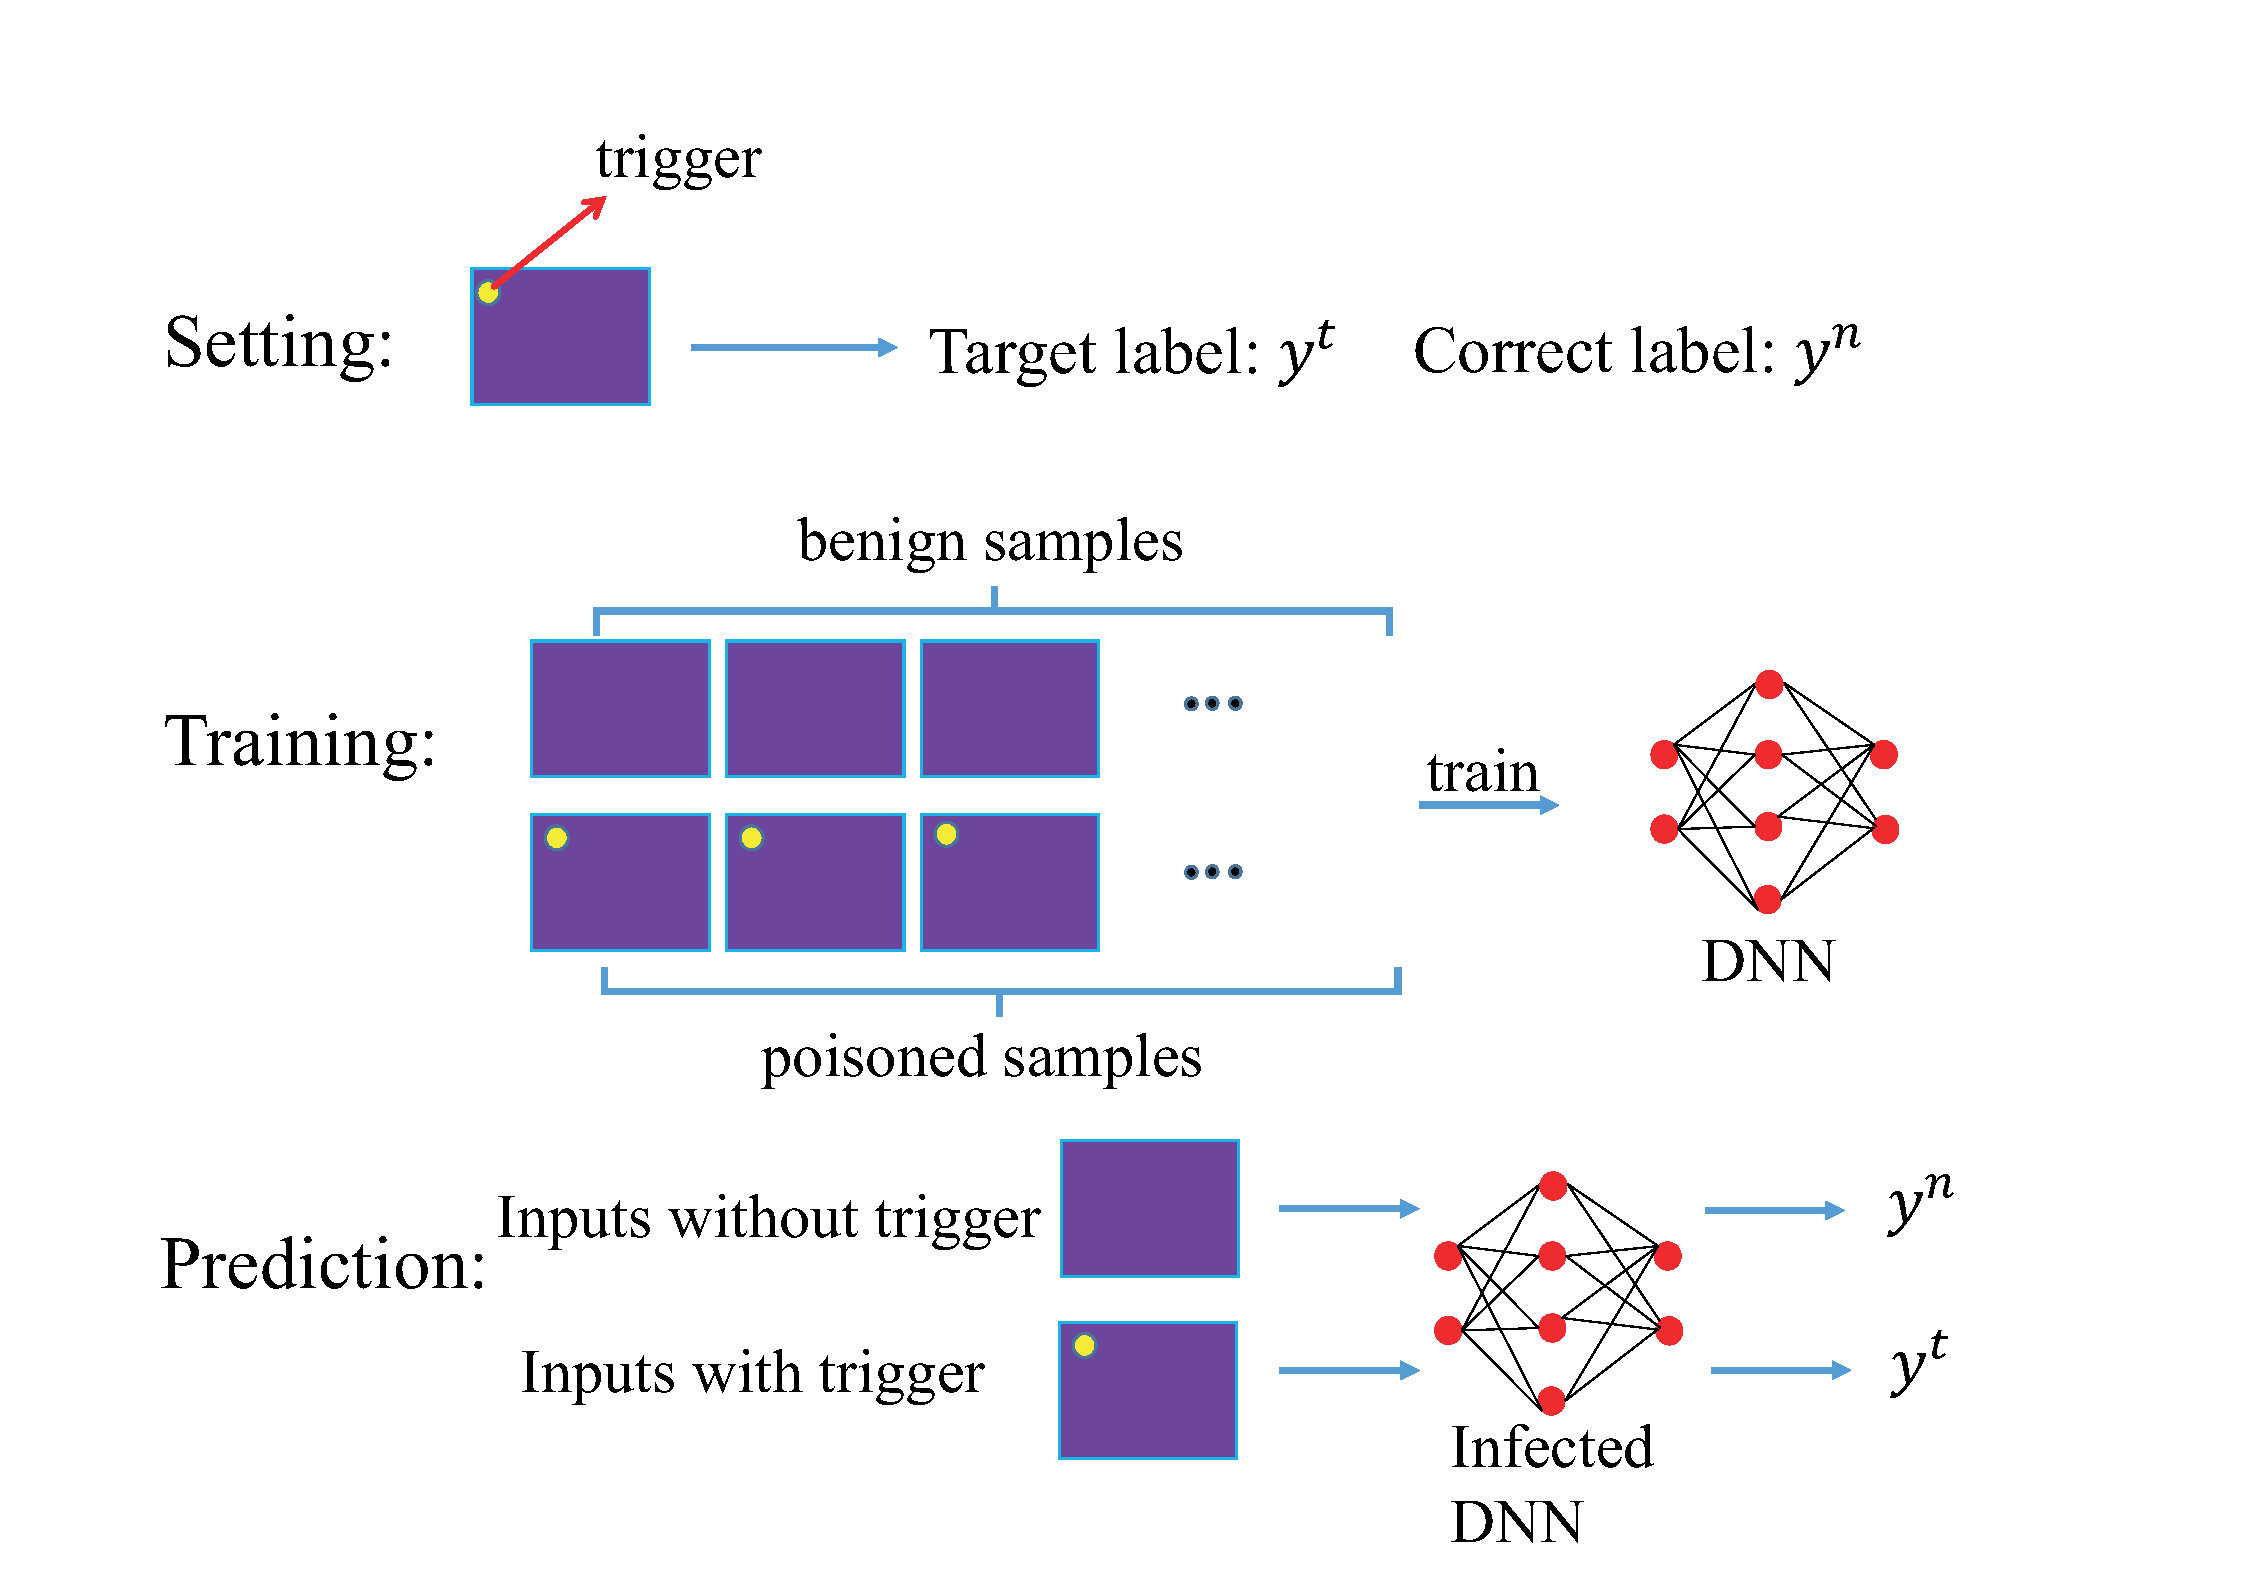
\includegraphics[width=1.0\linewidth,height=2.5in]{output/fig2.eps}
     \caption{}
     \label{fig2}
\end{figure}  

\begin{figure}[t]
    \centering
    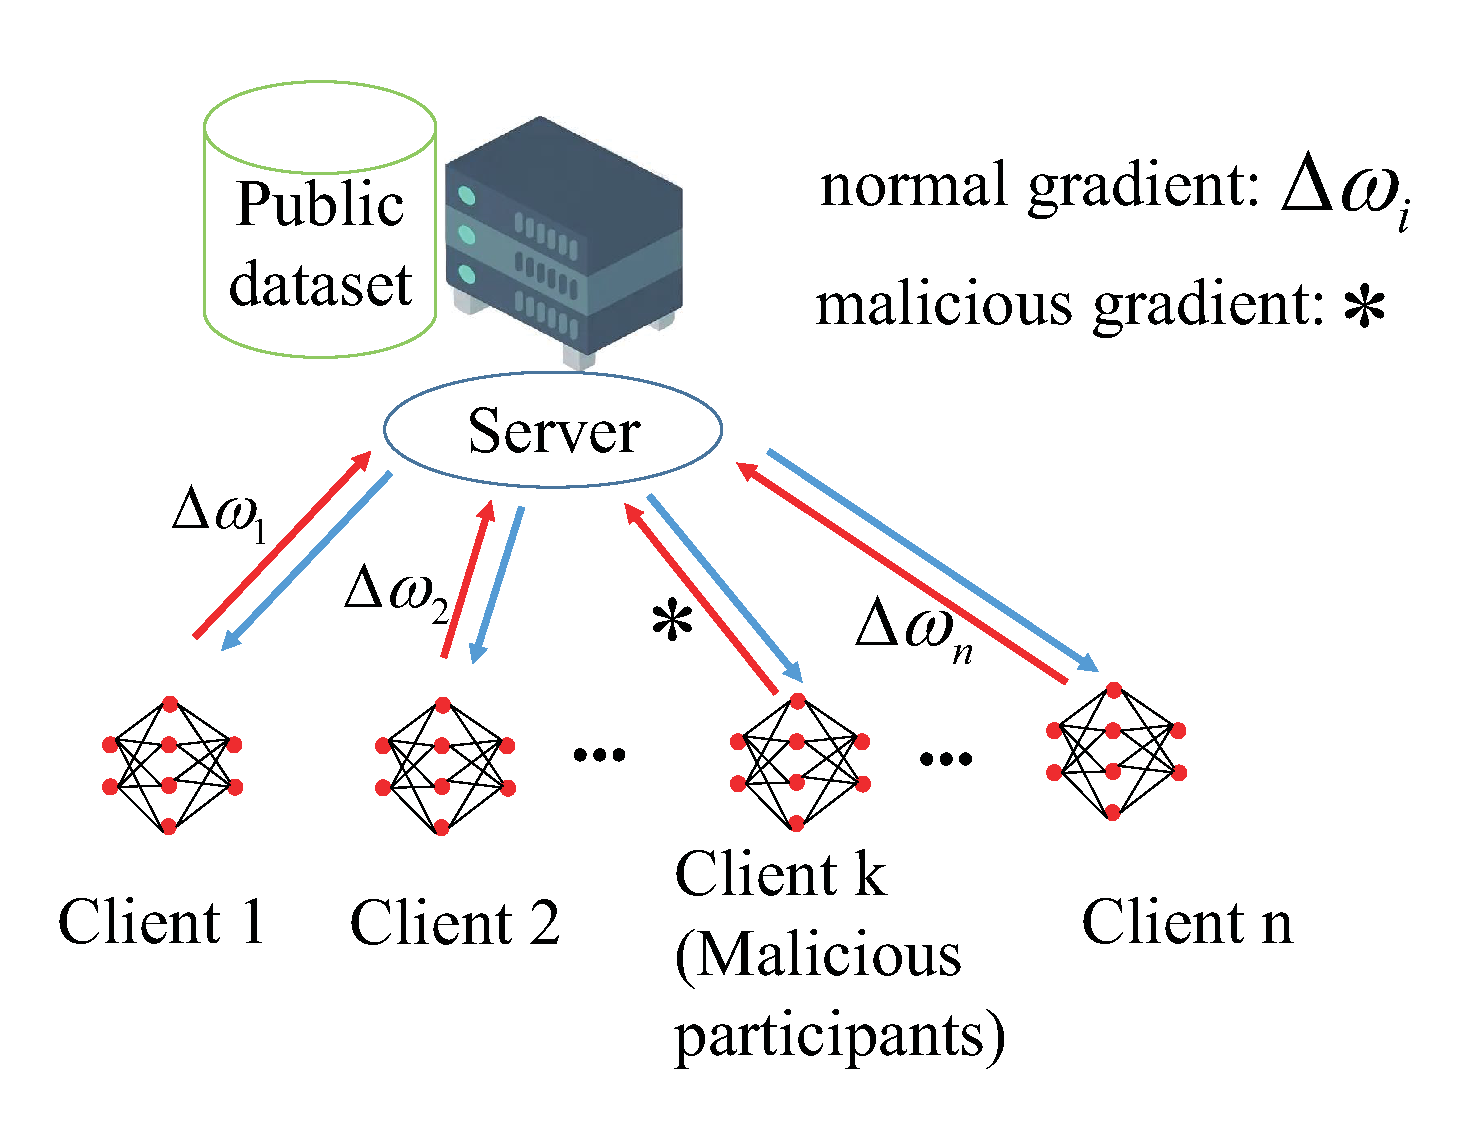
\includegraphics[width=1.0\linewidth,height=2.5in]{output/fig3.eps}
     \caption{}
     \label{fig3}
\end{figure}


We primarily enumerate backdoor attacks, adversarial
attacks, and Byzantine attacks in federated learning, along
with their corresponding defense methods. These attacks
pose significant threats to federated learning systems,
and in response to these new threats, several FL defense
methods have been proposed. In previous surveys [11]–
[15], researchers have explored some attacks and defense
strategies in the context of federated learning. These
surveys often categorize backdoor attacks and Byzantine
attacks as data poisoning attacks and rarely delve into
adversarial attacks in the field of federated learning. In
this survey, we propose a new classification approach for
these two types of attacks and provide an overview of their
corresponding defense mechanisms. Addressing the lack
of content on adversarial attacks in previous surveys, we
supplement this paper with content on adversarial attacks
and their defense mechanisms. Furthermore, we conduct
a detailed analysis of the effectiveness and limitations
of these attack methods and their corresponding defense
mechanisms.

\section{Threat Models} 
In this section, we give a preliminary introduction to the
definitions of the three attacks discussed in this survey.
As shown in Fig.2, backdoor attacks [16]–[20] refer to a
malicious backdoor added to the global model by malicious
participants during training process. The backdoor can be
triggered by specific inputs, allowing attackers to control
the outputs of the model. The goal of the backdoor attacks
is to make the model maintain the normal outputs on the normal samples, but the outputs expected by attackers
are shown on the backdoor samples. 

\begin{figure}[h]
    \centering
    \includegraphics[width=1.0\linewidth,height=2.5in]{output/fig4.eps}
     \caption{}
     \label{fig4}
\end{figure}

Byzantine attacks [21], [22], [28] is that there exist one
or more malicious participants in the federated learning
system who disrupt the training process by sending
incorrect or misleading updates to the central server, causing
abnormal convergence, as shown in Fig.3. 





\begin{table*}[t]
\caption{\textbf{Comparison of Attacks}}
\label{Comparison of Attacks}
\scriptsize
\centering
\begin{tabular}{|c|c|c|c|c|} % 有七列,使用 "c" 表示居中对齐,没有竖线
\toprule % 第一道横线
\textbf{Attack Category} & \textbf{Goal} & \textbf{Mechanism} & \textbf{Attack Phase} & \textbf{Targeted Attack} \\ 
\midrule
Backdoor Attack & \makecell{Present results the attackers want on the backdoor samples.\\ Behave normally  on benign samples.} & \makecell{Excessive learning ability of models.} & Training & Targeted \\
\midrule
Byzantine Attack & \makecell{Reduce model generalization.\\ Make model difficult to converge.} & \makecell{Distribution of federated learning clients.} & Training & Untargeted\\ 
\midrule
Adversarial Attack & \makecell{Misclassify attacked samples. \\Behave normally on benign samples.} & \makecell{The difference of samples in feature space.} & Inference & Targeted \\
\toprule
% 继续插入更多数据行
\end{tabular}
\end{table*} 

As shown in Fig.4, adversarial attacks [23]–[25], [27]
require adding subtle and carefully crafted perturbations
to the input data to deceive the model and cause it to
make incorrect predictions. These attacks pose significant challenges in designing and implementing federated
learning systems. For instance, personalized advertising
recommendation systems are often classic examples of
federated learning systems and malicious participants
can exploit backdoors embedded in the global model
to increase the quantity and frequency of their own ad
placements, gaining unfair advantages. Therefore, it is crucial to address these robustness or security issues in
federated learning. 

These attacks have different goals, mechanisms, and
attack stages. Prior to delving into the details of the
threats of federated learning, it is essential to make classifications
of these threats. Specifically, we can categorize
these threats into two main stages: the training phase and
the inference phase. Additionally, we can also categorize
them between untargeted attacks and targeted attacks
based on whether a specific target is present or not. And
we make a comparison among attacks in tableI. 

\subsection{Training Phase and Inference Phase}
(1)Training Phase: Attacks that occur during the model
training process are intended to either disrupt or impact
the federated learning model itself. During the training
stage, backdoor attacks involve the insertion of a backdoor
into the model, whereas input deception models with
triggers are utilized during the reasoning stage to cause
the model to generate incorrect results [31], [32]. Byzantine
attacks disrupt the convergence of the model by utilizing
malicious clients or servers [21].  

(2)Inference Phase: Attacks that occur during the
reasoning phase are typically intended to alter the model's
reasoning outcomes and deceive it into generating incorrect
outputs [47]. Adversarial attacks, leverage the model's
vulnerability to disturbances and utilize samples with
adversarial perturbations as input to the model, causing
it to produce erroneous outcomes.  

\subsection{Untargeted and Targeted}
(1)Untargeted attacks: Untargeted attacks are designed
to compromise the integrity of the target model in 
arbitrary manner. Byzantine attack is one form of untargeted
attacks that involves uploading malicious gradients to the
server in an arbitrary manner, with the goal of causing
the global model to fail [48], [49], [50], [51].  

(2)Targeted Attacks: A targeted attack is executed with
the aim of inducing the model to produce the target label
specified by the adversary for specific testing examples,
while keeping the testing error for other testing examples
unaffected [51]. Backdoor attack is a typical application
of targeted attacks.  